\documentclass[11pt]{article}
\usepackage{amsmath,textcomp,amssymb,geometry,graphicx,tikz,cancel}
\usepackage{algpseudocode,algorithm}

\def\Name{Zackery Field}  % Your name
\def\Sec{Di, 103}  % Your GSI's name and discussion section
\def\Login{cs170-fe} % Your login
\def\Homework{6}%Number of Homework, PUT SOMETHING HERE
\def\Session{Fall 2013}


\title{CS170--Fall 2013 --- Solutions to Homework 6}
\author{\Name, section \Sec, \texttt{\Login}}
\markboth{CS170--\Session\  Homework \Homework\ \Name, section \Sec}{CS170--\Session\ Homework \Homework\ \Name, section \Sec, \texttt{\Login}}
\pagestyle{myheadings}

\begin{document}
\maketitle

\section*{1. (10+5 pts.) Graph Construction}


A farmer(F) wants to cross the river with his wolf(W), sheep(S) and cabbage(C). F can carry at most one of W,S or C in the boat. Without the presence of F, W will eat S, and S will eat C. F can go back and forth across the river, and he wants to safely move all W, S, and C from the east side of the river (E) to the west side (W). One river crossing means the farmer goes from E to W, or W to E.
\begin{itemize}
\item[] {\bf (a)} Find a solution involving the least number of river crossings for the farmer.

We can construct a graph that traverses the space of possible crossings. $W[] $ and $ E[] $ describe everything on the west and east side respectively after the move, including the presence of the farmer. If there is a configuration that breaks a rule, then the children of that vertex are not explored.

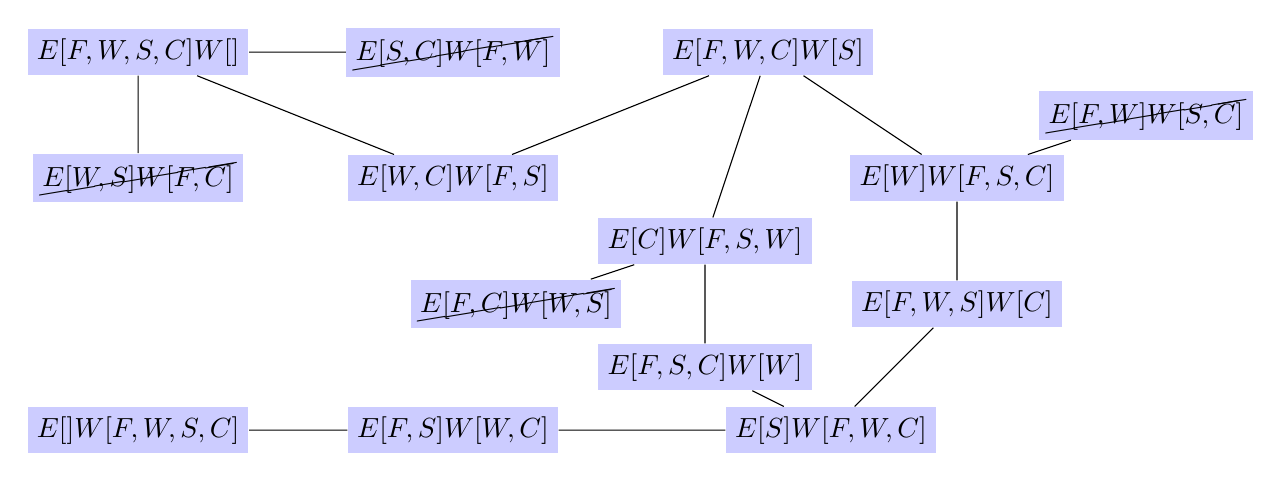
\begin{tikzpicture}
  [scale=.8,auto=left,every node/.style={rectangle,fill=blue!20}]
  \node (init) at (-2,10) {$E[F,W,S,C]W[]$};
  \node (1wolf) at (3,10)  {$\cancel{E[S,C]W[F,W]}$};
  \node (1cab) at (-2,8)  {$\cancel{E[W,S]W[F,C]}$};
  \node (1sheep) at (3,8)  {$E[W,C]W[F,S]$};
  \node (sheep) at (8,10)  {$E[F,W,C]W[S]$};
  % First break decision
  \node (2cab) at (11,8) {$E[W]W[F,S,C]$};
  \node (2wolf) at (7,7) {$E[C]W[F,S,W]$};
  % Continue after break decision
  \node (backsheep_cab) at (11,6) {$E[F,W,S]W[C]$};
  \node (backsheep_wolf) at (7,5) {$E[F,S,C]W[W]$};
  \node (nosheep_cab) at (14,9)  {$\cancel{E[F,W]W[S,C]}$};
  \node (nosheep_wolf) at (4,6)  {$\cancel{E[F,C]W[W,S]}$};
  % Converge back to W,C and sheep alone
  \node (converge) at (9,4) {$E[S]W[F,W,C]$};
  \node (between) at (3,4) {$E[F,S]W[W,C]$};
  \node (final) at (-2,4) {$E[]W[F,W,S,C]$};
 
  \foreach \from/\to in {init/1sheep,init/1wolf,init/1cab,1sheep/sheep,
  						sheep/2cab,sheep/2wolf,
  						2wolf/backsheep_wolf,2cab/backsheep_cab,
              2wolf/nosheep_wolf,2cab/nosheep_cab,
              backsheep_wolf/converge, backsheep_cab/converge,
              converge/between,between/final}
    \draw (\from) -- (\to);

\end{tikzpicture}

All of the paths are undirected because there is no reason why the farmer could not move back and forth between two configurations, although it would be useless. The minimum solution is then 7 total crossings.
\end{itemize}
\label{pg:end-of-p1}
% Make sure that the solution here does not exceed one page here. If
% it does, use the extra space for this problem at the end.  
%
% Comment out the next line if you are NOT using the extra space
\paragraph{} \emph{Continued on Page \pageref{pg:p1-continuation}}
\newpage


%%Do NOT remove/comment the next line
\pagestyle{plain}
%%It makes sure your name appears only on the first page
\section*{2. (15 pts.) Trip}
In a country with $n$ cities, we have two methods of travel: roads and planes. (more formally, our graph is $G = (V,R\cup P)$, where $V$ is our set of cities, $R$ is the set of roads, and $P$ are the set of planes). Roads $i$ is specified as an undirected edge ($u_i,v_i,C_i$) that connects the two cities $u_i,v_i$ with a non-negative cost $C_i$. Planes $j$ specified as directed edges ($u_j,v_j,C_j$) which connects city $u_j$ to $v_j$ (one way) with cost $C_j$ (Due to some weird airline award program, the cost can possibly be negative!) with the additional constraint that there is no sequence of roads and planes that we can follow that takes us back from $v_j$ to $u_j$.
Assume we have the the adjacency list representation of roads and planes (two separate data structures), and we can freely swap between the two methods of travel (i.e. we can take an arbitrary amount of roads, then planes, then roads, and so on...).
Given two cites $s$,$t$, give an efficient algorithm to compute the shortest path from $s$ to $t$ (should have same running time as Dijkstra).

We can construct a new graph where each of the undirected edges $r_{u,v}\in R$ can be decomposed into two directed edges $r_{u\rightarrow v}$ and $r_{v\rightarrow u}$. Each of these new edges maintain the original edge weight of $r_{u,v}$. Since we are guranteed that there is no sequence of roads and planes that we can follow that takes us back from $v_j$ to $u_j$, we can topologically sort the graph. As described in Figure 4.15, we can visit each vertex $u\in V$ in sorted order and update the edges (with respective costs $C_{i/j}$) along the way to all other nodes. After this we are given the minimal distance from city $s$ to all other cities $\in V$ and we can simply lookup the distance between $s$ and $t$. If we want to also know the path from $s$ to $t$ with certainty (and not just distance), then we will have to store each path as the graph is searched.

This algorithm thusfar is guranteed to run in linear time. Linearization of $G$ takes linear time and so does visiting each vertex $\in V$ and updating each edge distance. To get the actual path from $s$ to $t$ will take a bit more searching, and possibly a lot of memory. In order to find the path, start from $t$ and subtract the edge costs of all edges incoming to $t$ and see follow the path back to $s$ that has the lowest path length from $s$ to $t-i$. You are guranteed to have the minimal path length at each step because when the algorithm was run forward you updated each of these paths with all available information. This path traceback will also take linear time. So the total running time of the algorithm is $O((|E|+|V|)\log|V|)$ with a binary heap.

\label{pg:end-of-p2}
% Make sure that the solution here does not exceed one page here. If
% it does, use the extra space for this problem at the end.  
%
% Comment out the next line if you are NOT using the extra space
\paragraph{} \emph{Continued on Page \pageref{pg:p2-continuation}}



\newpage

\section*{3. (10+5 pts.) Shortest path in currency trading}

\begin{itemize}
\item[] {\bf (a)} Give an efficient algorithm for the following problem: Given a set of exchange rates $r_{i,j}$ (describes $c_i\rightarrow c_j$), and two currencies $s$ and $t$, find the most advantageous sequence of currency exchanges for converting currency $s$ into currency $t$. Toward this goal, you should represent the currencies and rates by a graph whose edge lengths are real numbers.

If ${r_{i,j}}_b < {r_{i,j}}_a < 1$ then ${r_{i,j}}_a$ is the better exchange rate from $c_i$ to $c_j$ because it has a lower transaction fee. The most advantageous sequence then contains path with the greatest total edge weight product: $\mbox{MAX}(\Pi_{i\not= j}{r_{i,j}})$.  We can apply Dijkstra's algorithm to calculate these sums, and instead of relaxing each vertex based on minimum edge weight we can relax each vertex based maximum edge weight. This will effectively give us the maximum of every path from $s$ to $t$ and will return the path that yields the maximum value $c_t$. This algorithm is trivially different from Dijkstra's and the proof of Dijkstra's (in the book) is sufficient to prove its correctness. Because $|E| >> |V|$ (we can transact between any two currencies; weighted complete graph) we can use a Fibonacci heap in our implementation to restrict the runtime to: $O(|E| + |V|\log|V|)$. Yes, the Fibonacci heap may be difficult to implement, but when it comes to matters of large sums of money it should be worth it.

Note: As stated in a piazza post $r_{i,j}$ are all strictly poistive. 

\item[] {\bf (b)} Give an efficient algorithm for detecting the presence of such an anomaly. Use the graph representation you found above. 

Start by doing an $O(|V|+|E|)$  DFS or BFS search looking for an $r_{i,j} > 1$. If there is no such $r_{i,j}$ then there is (trivially) no anomaly, return false. Collect all of the edge weights $r_{i,j} > 1$, and let this collection be called $E'$. If $|E'| = |E|$, then we know that there is an anomaly, because any cycle in the currency graph will yield $r_{i_{1}i_{2}}*\cdots*r_{i_{k}i_{1}}>1$, return true.

For the case of $1\leq|E'|<|E|$, you can run Dijkstra's a number of times starting at all currencies that correspond to the start vertex of each $e\in E'$ and return true upon finding an $r_{i_{1}i_{2}}*\cdots*r_{i_{k}i_{1}}>1$. Return false, if after a search of all $e \in E'$ you do not find $r_{i_{1}i_{2}}*\cdots*r_{i_{k}i_{1}}>1$. It is true that the search must contain at least one $e\in E$ or else the product $r_{i_{1}i_{2}}*\cdots*r_{i_{k}i_{1}}\leq1$. Since each run of Dijkstra's (using Fibonacci heap) takes $O(|E| + |V|\log|V|)$ and we run the algorithm at maximum $|E|-1$ times the bounded running time is: $O(|E|^2+|E||V|\log|V|)$
\end{itemize}
\label{pg:end-of-p3}



% Make sure that the solution here does not exceed one page here. If
% it does, use the extra space for this problem at the end.  
%
% Comment out the next line if you are NOT using the extra space
% \paragraph{} \emph{Continued on Page \pageref{pg:p3-continuation}}

\newpage

\section*{4. (5+5+5+5 pts.) Cycle property, another MST algorithm}

{\bf Property: }Pick any cycle in the graph, and let e be the heaviest edge in that cycle. Then there is a minimum spanning tree that does not contain e.

\begin{itemize}
\item[] {\bf (a)} Prove this property carefully.

The (heaviest) edge $e\in E$ of the graph $G=(V,E)$ is in a cycle in $G$. Assume for the sake of contradiction that $e\in E'$, where $T=(V,E')$ is a MST of $G$. 
Since $e$ is in a cycle, $|E'| < |E|$. This is follows from the definition of MST, more specifically, any $T$ will not contain any cycles because at least one of the edges in such a cycle could be removed and each vertex $\in V$ could still be reached. From this realization, we know that there must have been some other edge $e' \in E$ that was a part of the same cycle as $e$. We also know that, $\forall e': w_{e'}<w_{e}$, so $e'$ would have been placed in the MST in place of $e$ in order to satisfy the minimization condition of MSTs. This a contradiction, since we assumed that $e\in E'$. $\square$  
\item[] {\bf (b)} Here is the new MST algorithm. 

The input is some undirected graph $G = (V, E)$ (in adjacency list format) with edge weights $\{w_e\}$.

  \begin{algorithmic}
  \State sort the edges according to their weights
  \For {each edge $e \in E$, in decreasing order of $w_e$}
    \If {$e$ is part of a cycle of $G$: $G.pop(e)$}\EndIf
  \EndFor
  \State return G
  \end{algorithmic}

Prove that this algorithm is correct.

We want to show that by removing all cycles from $G$ by deleting edges in decreasing order then we will arrive at a MST of $G$. To start, all cycles must be removed from $G$. If any cycles remain in the MST of $G$ then we know that at least one of the edges of the cycle can be removed while still maintaining the connectivity of $G$. All that remains is to show that removal of edges based on decreasing edge weights is the appropriate order of removal. Let $E_{keep}$ be the set of edges that remains in the MST of $G$ and let $E_{toss}$ be the set of edges that is deleted in the MST description of $G$. In order to satisfy the minimization condition of a MST, we know that for each edge $e_{keep} \in E_{keep}$ and for each edge $e_{toss} \in E_{toss}$: $e_{keep}<e_{toss}$ (if they are part of the same cycle). Removing edges in $e \in E$ in decreasing order is one way to ensure that this inequality holds for all $e\in E_{keep}$ and for all $e\in E_{toss}$. $\square$
\end{itemize}
\label{pg:end-of-p4}

% Make sure that the solution here does not exceed one page here. If
% it does, use the extra space for this problem at the end.  
%
% Comment out the next line if you are NOT using the extra space
\paragraph{} \emph{Continued on Page \pageref{pg:p4-continuation}}


\newpage

\section*{5. (5+5+5+5 pts.) Update MST after changing one edge}

You are given a graph $G = (V,E)$ with positive edge weights, and a minimum spanning tree $T = (V, E')$ with respect to these weights; you may assume $G$ and $T$ are given as adjacency lists. Now suppose the weight of a particular edge $e \in E$ is modified from $w(e)$ to a new value $\hat{w}(e)$. You wish to quickly update the minimum spanning tree $T$ to reflect this change, without recomputing the entire tree from scratch. 
\begin{itemize}
  \item[] \textbf{(a)} $e \not\in E'$ and $\hat{w}(e) > w(e)$

  This case is trivial. It is the case that $e \not\in E'$, because there was some other edge $e'\in E'$ s.t. $w_{e'}<w_{e}$ and $e'$ satisfied the connectivity of $G$. Since $\hat{w}(e) > w(e)$ the inequality  $w_{e'}<w_{e}$ is maintained, and so $e$ continues to not be in $E'$, in order to maintain the minimization constraint of MSTs. $\square$
  \item[] \textbf{(b)} $e \not\in E'$ and $\hat{w}(e) < w(e)$

  For this case we will need to check that $e$ does not replace some $e'\in E'$. If in the original graph $G$, $e$ and $e'$ are in the same cycle and $\hat{w}(e)<w(e')<w(e)$, then we will need to update $T$ to remove $e'$ and replace it with $e$. Start a DFS from one of the vertices bounding $e$ and do pre and post markings of each vertex. If for any pre and post number configuration satisfying $pre(v)<pre(u)<post(u)<post(v)$ for an edge $e=(u,v)$ then that edge is in a cycle. Since $e$ is in a cycle, it is a possibility that $\exists e'$ s.t. $\hat{w}(e)<w(e')<w(e)$. So we only need to check if this is the ineqaulity holds (by travelling around the cycle), and we can replace this $e'$ (with the largest edge weight) by the edge $e$ s.t. $w(e)<w(e')<\hat{w}(e)$ is satisfied. $\square$ Note: running time on extra page.
  \item[] \textbf{(c)} $e \in E'$ and $\hat{w}(e) < w(e)$

  As with (a), this case is also trivial. It is the case that $e \in E'$, because for all other edges $e'\not\in E'$ that maintain the same connectivity as $e$ (i.e. both in the same cycle), $w_{e'}>w_{e}$. Since $\hat{w}(e) < w(e)$ the inequality  $w_{e'}>w_{e}$ is maintained, and so $e$ continues to be in $E'$, in order to satisfy the minimization constraint on MSTs. $\square$ 

\end{itemize}
\label{pg:end-of-p5}


% Make sure that the solution here does not exceed one page here. If
% it does, use the extra space for this problem at the end.  
%
% Comment out the next line if you are NOT using the extra space
\paragraph{} \emph{Continued on Page \pageref{pg:p5-continuation}}


\newpage


% \section*{Problem 6}

% \subsection*{Part (a)}
% \subsection*{Part (b)}

% \label{pg:end-of-p6}

% % Make sure that the solution here does not exceed one page here. If
% % it does, use the extra space for this problem at the end.  
% %
% % Comment out the next line if you are NOT using the extra space
% \paragraph{} \emph{Continued on Page \pageref{pg:p6-continuation}}


\newpage


%% Comment out the "extra spaces" completely for the problems for you
%% don't need them

\section*{Extra space for Problem 1}
\emph{Continued from Page \pageref{pg:end-of-p1}}\\


\label{pg:p1-continuation}

Graph repeat:


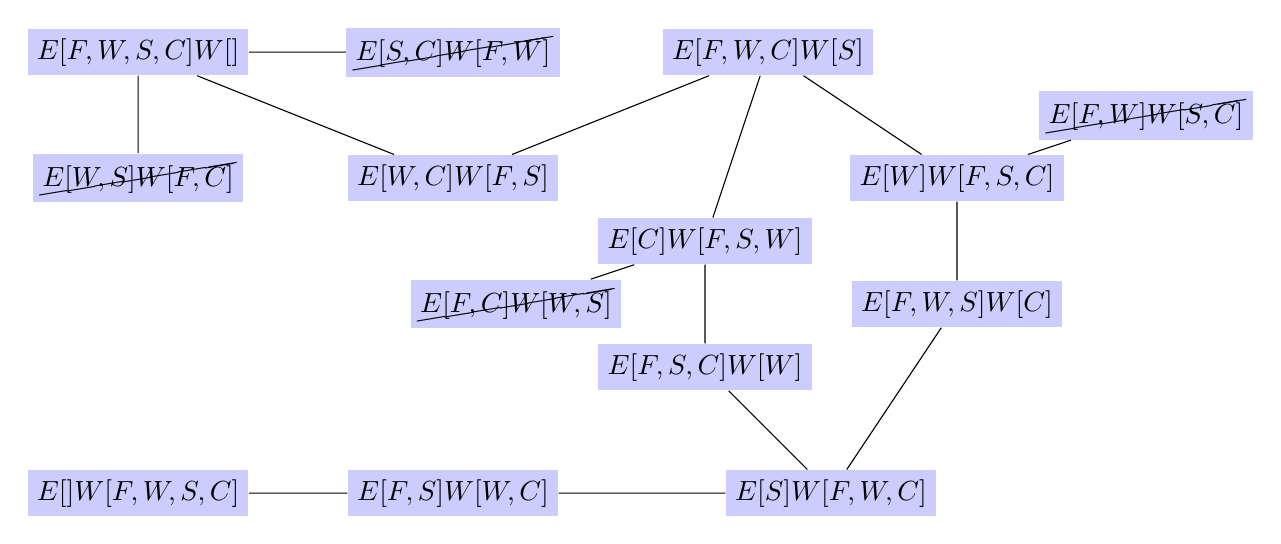
\begin{tikzpicture}
  [scale=.8,auto=left,every node/.style={rectangle,fill=blue!20}]
  \node (init) at (-2,10) {$E[F,W,S,C]W[]$};
  \node (1wolf) at (3,10)  {$\cancel{E[S,C]W[F,W]}$};
  \node (1cab) at (-2,8)  {$\cancel{E[W,S]W[F,C]}$};
  \node (1sheep) at (3,8)  {$E[W,C]W[F,S]$};
  \node (sheep) at (8,10)  {$E[F,W,C]W[S]$};
  % First break decision
  \node (2cab) at (11,8) {$E[W]W[F,S,C]$};
  \node (2wolf) at (7,7) {$E[C]W[F,S,W]$};
  % Continue after break decision
  \node (backsheep_cab) at (11,6) {$E[F,W,S]W[C]$};
  \node (backsheep_wolf) at (7,5) {$E[F,S,C]W[W]$};
  \node (nosheep_cab) at (14,9)  {$\cancel{E[F,W]W[S,C]}$};
  \node (nosheep_wolf) at (4,6)  {$\cancel{E[F,C]W[W,S]}$};
  % Converge back to W,C and sheep alone
  \node (converge) at (9,3) {$E[S]W[F,W,C]$};
  \node (between) at (3,3) {$E[F,S]W[W,C]$};
  \node (final) at (-2,3) {$E[]W[F,W,S,C]$};
 
  \foreach \from/\to in {init/1sheep,init/1wolf,init/1cab,1sheep/sheep,
              sheep/2cab,sheep/2wolf,
              2wolf/backsheep_wolf,2cab/backsheep_cab,
              2wolf/nosheep_wolf,2cab/nosheep_cab,
              backsheep_wolf/converge, backsheep_cab/converge,
              converge/between,between/final}
    \draw (\from) -- (\to);

\end{tikzpicture}
\begin{itemize}

\item[] {\bf (b)} How many different such solutions (i.e. with least number of crossings) are there?

There are two such solutions with the least number of crossings (7 crossings). At minimum. If there were no restrictions the farmer could find a solution in 5 crossings. The restriction on who eats who forces the farmer to make an extra trip to isolate the sheep (either by leaving it one side alone or keeping it in his presence), which requires 5+2 crossings. Graphically, if the crossed out paths continued, there would be a 5 crossing solution.
\end{itemize}

\newpage
%%Comment out the above three lines if you are not using extra space
%%for this problem.


\section*{Extra space for Problem 2}
\emph{Continued from Page \pageref{pg:end-of-p2}}\\

%Insert solution here

\label{pg:p2-continuation}
\newpage
%%Comment out the above three lines if you are not using extra space
%%for this problem.


% \section*{Extra space for Problem 3}
% \emph{Continued from Page \pageref{pg:end-of-p3}}\\

% %Insert solution here

% \label{pg:p3-continuation}
% \newpage
%%Comment out the above three lines if you are not using extra space
%%for this problem.



\section*{Extra space for Problem 4}
\emph{Continued from Page \pageref{pg:end-of-p4}}\\

\begin{itemize}
\item[] {\bf (c)} On each iteration, the algorithm must check whether there is a cycle containing a specific edge $e$. Give a linear-time algorithm for this task, and justify its correctness.

Do a DFS starting from one of the vertices $v$ on $e$ marking all vertices when they are popped off the stack, or more generally, mark when visited. If you come across a vertex that is marked then you know that it is in a cycle. A DFS search will only visit a vertex twice if it is in a cycle (proven in book). A DFS search also takes $O(|V| + |E|)$
 time (also shown in book). $\square$

 \item[] {\bf (d)} What is the overall time taken by this algorithm, in terms of $|E|$? Explain your answer. 

For each of the vertices $e\in E$, in decreasing order, we have to do a linear-time cycle search (DFS) on each of them for a total running time of: $O(|E|(|V|+|E|))$. $\square$
\end{itemize}

\label{pg:p4-continuation}
\newpage
%%Comment out the above three lines if you are not using extra space
%%for this problem.



\section*{Extra space for Problem 5}
\emph{Continued from Page \pageref{pg:end-of-p5}}\\

\begin{itemize}
  \item[] \textbf{(d)} $e \in E'$ and $\hat{w}(e) > w(e)$

   For this case we will need to check that $e$ does not get replaced by some $e'\not\in E'$. If in the original graph $G$, $e$ and $e'$ are in the same cycle and $w(e)<w(e')<\hat{w}(e)$, then we will need to update $T$ to remove $e$ and replace it with $e'$. Start a DFS from one of the vertices bounding $e$ and do pre and post markings of each vertex. If for any pre and post number configuration satisfying $pre(v)<pre(u)<post(u)<post(v)$ for an edge $e=(u,v)$ then that edge is in a cycle. Since $e$ is in a cycle, it is a possibility that $\exists e'$ s.t. $w(e)<w(e')<\hat{w}(e)$. So we only need to check if this is inequality holds (by travelling around the cycle), and we can replace $e$ by the edge $e'$ with the smallest edge weight that still satisfies $w(e)<w(e')<\hat{w}(e)$. $\square$
  \item[] \textbf{running times}

   For (a) and (c), no updates need to be done and therefore they will run in $O(1)$ time. For both (b) and (c) you are doing a DFS which runs in $O(|V|+|E|)$ time and then iterating through the edges in any identified cycles checking for truth of the respective inequalities which takes at most $O(|E|+|V|)$ time. Then updating the adjacency list of $T$ can be done in at most $O(|E|)$ (in the case that the vertex that you are updating is well connected). So for (b) and (d) the running time is linear: $O(|V|+|E|)$.

\end{itemize}
\label{pg:p5-continuation}
\newpage
%%Comment out the above three lines if you are not using extra space
%%for this problem.


% \section*{Extra space for Problem 6}
% \emph{Continued from Page \pageref{pg:end-of-p6}}\\


% %Insert solution here


% \label{pg:p6-continuation}
% \newpage
% %%Comment out the above three lines if you are not using extra space
% %%for this problem.



\end{document}
